\documentclass[spanish]{beamer}
\usepackage[ansinew]{inputenc} % Acepta caracteres en castellano
\usepackage[spanish]{babel}    % silabea palabras castellanas
\usepackage{amsmath}
\usepackage{amsfonts}
\usepackage{amssymb}
\usepackage{dsfont}
\usepackage{graphicx}
\usepackage{geometry}
\usetheme{Madrid}
\usecolortheme{beaver}
\usepackage{textpos}
% Logo  en el comienzo 
\addtobeamertemplate{frametitle}{}{%
\begin{textblock*}{100mm}(.85\textwidth,-1cm)
{\includegraphics[height=0.4in, keepaspectratio=true]{/Users/luisnunez/Dropbox/MisDocumentos/UIS/UISImagenInstitucional/UISLOGO.png}}
\end{textblock*}}

\begin{document}

\title{\textbf{Coordenadas Generalizas} }
\author[L.A. N��ez]{\textbf{Luis A. N��ez}}  
\institute[UIS]{\textit{Escuela de F�sica, Facultad de Ciencias, } \\
\textit{Universidad Industrial de Santander, Santander, Colombia } \\
{\includegraphics[height=0.4in, keepaspectratio=true]{/Users/luisnunez/Dropbox/MisDocumentos/UIS/UISImagenInstitucional/UISLOGO.png}}
}
\date{\today}
\maketitle


\begin{frame}
\frametitle{Agenda}
  \tableofcontents
\end{frame}


%%%%% Diapo 1
\section{Coordenadas Generalizadas}
\frame{
  \frametitle{Coordenadas Generalizadas}
   \begin{itemize}  
  	\item<1-> Consideremos un sistema de N part�culas, $i = 1, 2, . . . , N$ , con vectores posici�n son ${{\bf r}_1, {\bf r}_2, . . . , {\bf r}_N }$ tal que ${\bf r}_i = (x_i, y_i, z_i)$. El sistema est� descrito por 3N coordenadas.
  	\item<2-> Pueden existir restricciones, ligaduras o v�nculos entre coordenadas, i.e. relaciones algebraicas o funcionales entre coordenadas: $f_1({\bf r}_1,{\bf r}_2,...,t) = 0, \; f_2({\bf r}_1,{\bf r}_2,...,t) = 0,  \cdots f_k({\bf r}_1,{\bf r}_2,...,t)$, 
  	\item<3-> Por ejemplo, el movimiento ocurre sobre un plano ($z = cte$), o sobre un c�rculo ($x^2 + y^2 = cte$), sobre una esfera ($x^2 +y^2 +x^2 = cte$), etc. 
	\item<4-> La cantidad $s = 3N -k$ es el n�mero de {\bf grados de libertad del sistema}, o el n�mero m�nimo de coordenadas independientes necesarias para describir el movimiento del sistema. 
	\item<5-> Los grados de libertad definen las {\bf coordenadas generalizadas},  $\{ q(t)_1, q(t)_2, . . . , q(t)_s\}$. 
	\item<6-> La evoluci�n temporal de estas coordenadas definen las {\bf velocidades generalizadas} $\{ \dot{q}(t)_1, \dot{q}(t)_2, . . . , \dot{q}(t)_s\}$. 
	\item<7-> En Mec�nica Cl�sica, el tiempo $t$ es un par�metro. 
    \end{itemize}
}
%%%%% Diapo 2
\section{V�nculos hol�nomos y no hol�nomos}
\frame{
  \frametitle{V�nculos hol�nomos y no hol�nomos}
  \begin{itemize}  
  	\item<1-> Los v�nculos hol�nomos son funciones de las coordenadas generalizadas y, posiblemente, del tiempo $f_i(q_1, q_2, \dots, q_N, t) = 0$. 
	\item<2->Estas restricciones reducen el n�mero de coordenadas independientes.
	\item<3-> En un p�ndulo simple de longitud $l$, la posici�n de la masa en coordenadas \((x, y)\) debe satisfacer la restricci�n: $x^2 + y^2 - l^2 = 0$, reduciendo los grados de libertad de dos a uno.
	\item<4-> Los v�nculos hol�nomos son integrables y permiten describir el movimiento del sistema con menos coordenadas.
	\item<5-> Los v�nculos no hol�nomos son $g(q_1, q_2, \dots, q_n, \dot{q}_1, \dot{q}_2, \dots, \dot{q}_n, t) \leq 0$ o tambi�n $g(q_1, q_2, \dots, q_n, \dot{q}_1, \dot{q}_2, \dots, \dot{q}_n, t) = 0$
	\item<6-> En un disco que rueda sin deslizar sobre un plano se tiene una restricci�n que involucra las velocidades del centro de masa y la velocidad angular: $ \dot{x}_{cm} - R\dot{\theta} = 0$.
	\item<7-> Los v�nculos no hol�nomos no pueden integrarse e involucran relaciones entre coordenadas y velocidades. 

   \end{itemize}
}
%%%%% Diapo 3
\section{Ejemplos}
\frame{
  \frametitle{Ejemplos}
			\begin{figure}[t]
			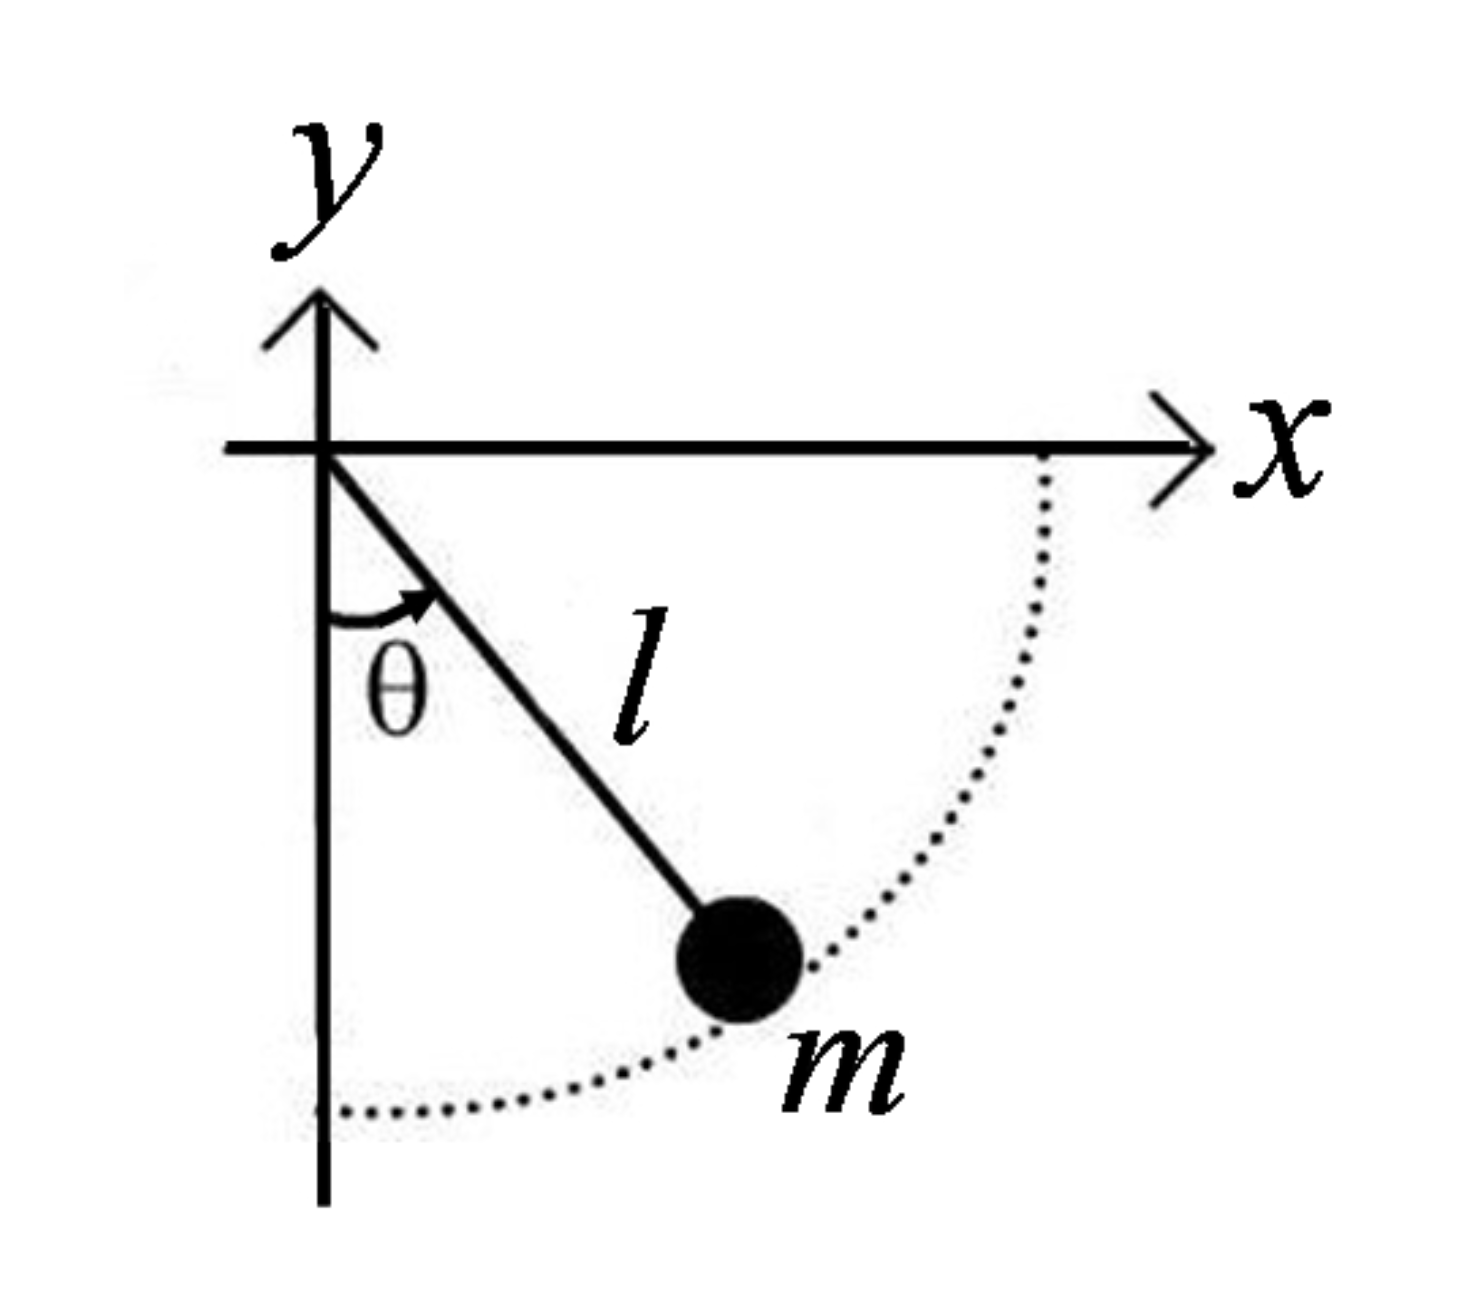
\includegraphics[width=1.4in]{Figuras/Pendulo.png} \hspace{1cm} 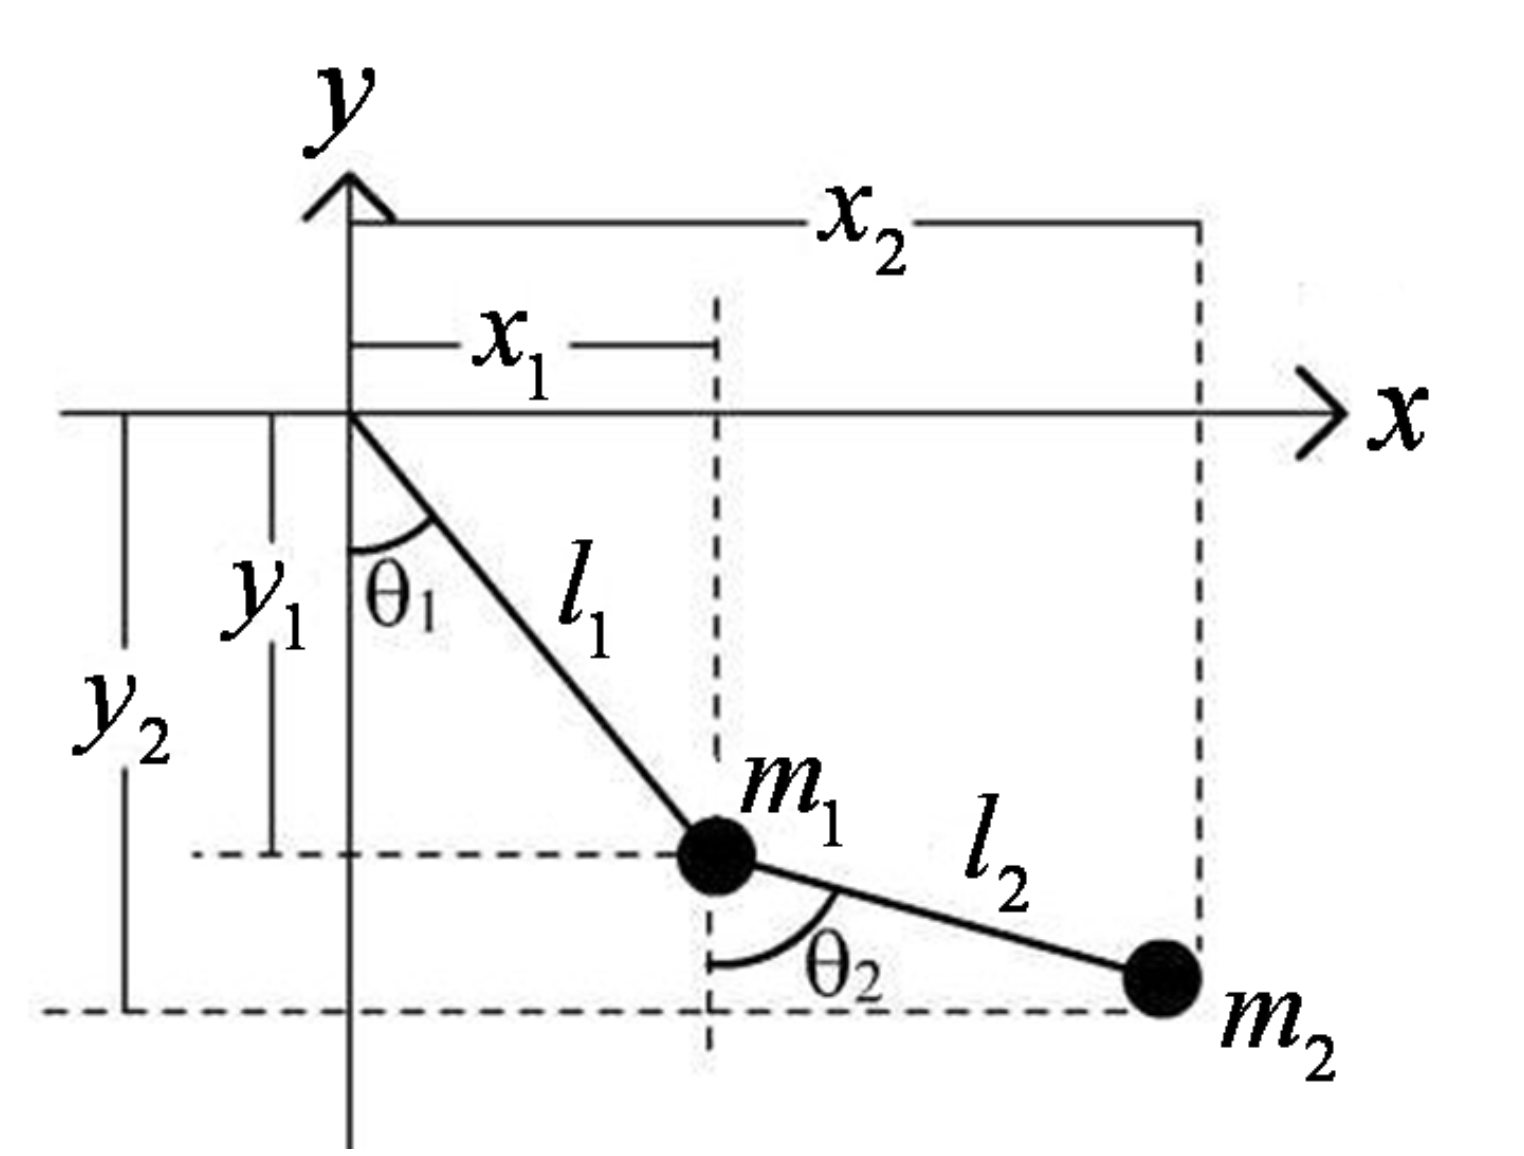
\includegraphics[width=1.4in]{Figuras/PenduloDoble.png} \\ 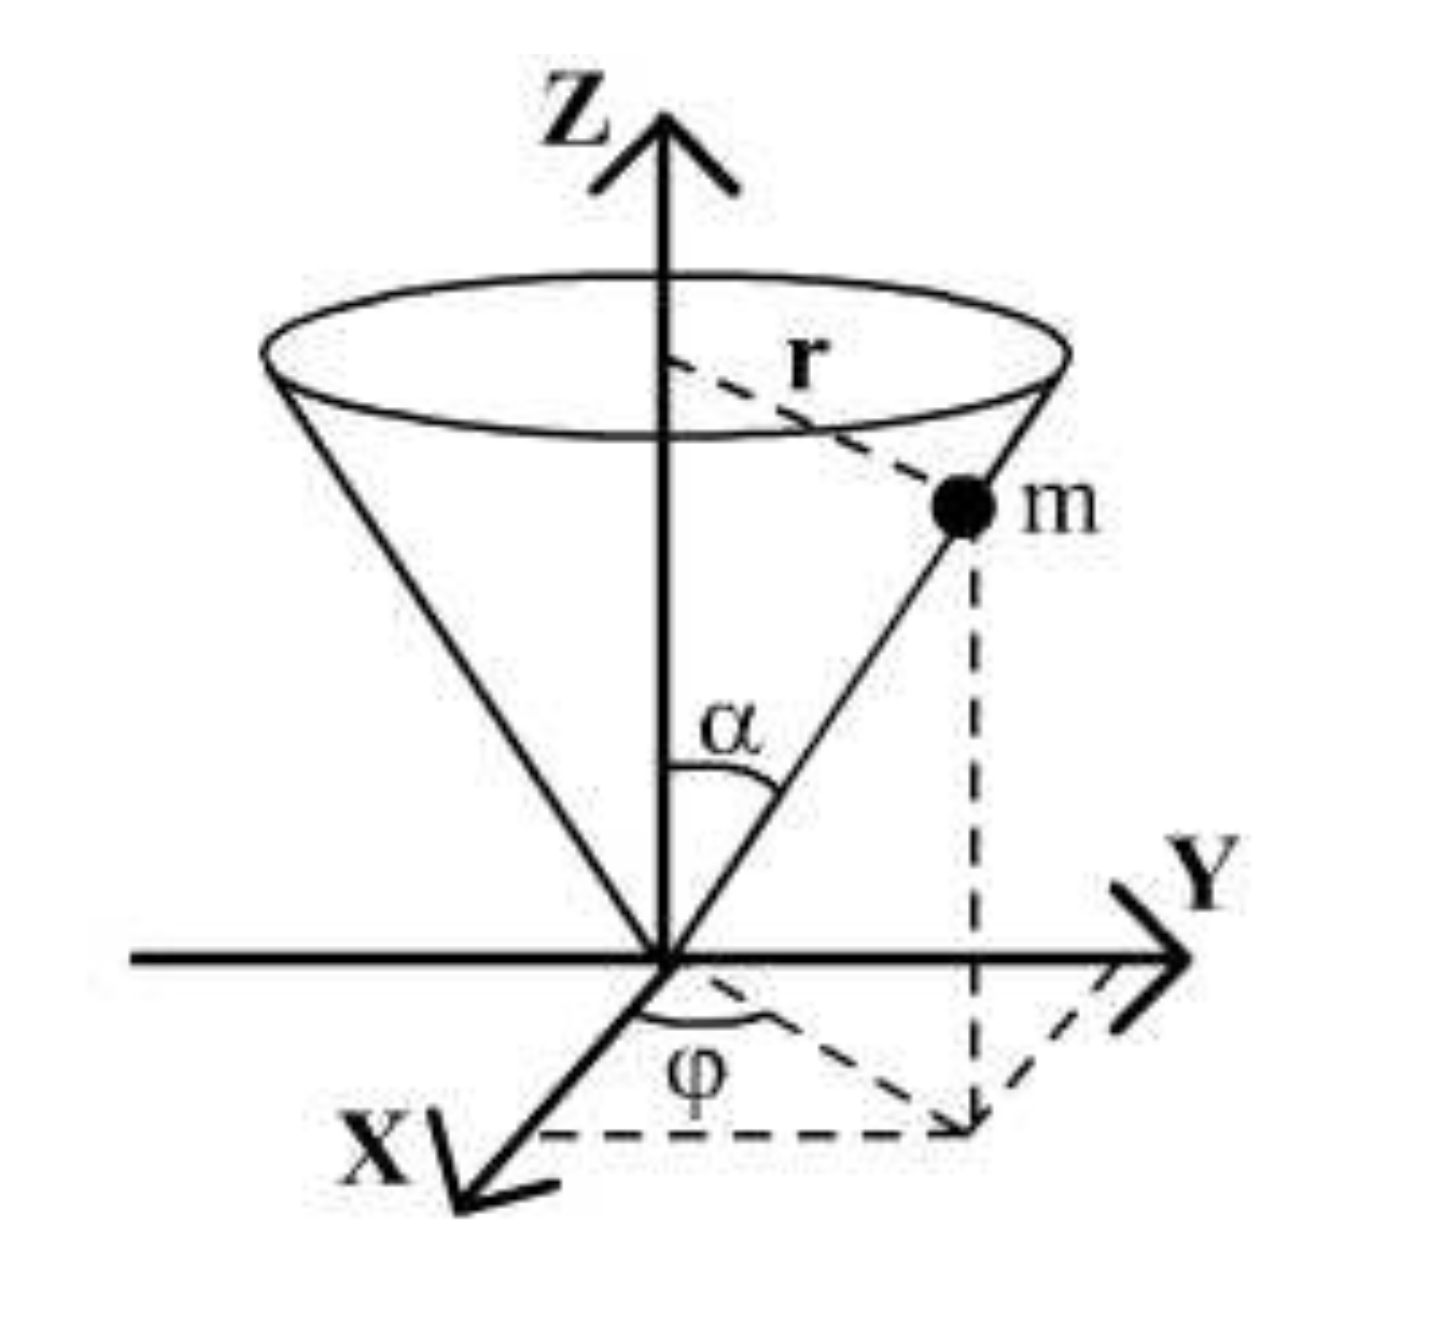
\includegraphics[width=1.4in]{Figuras/Cono.png} \hspace{1cm} 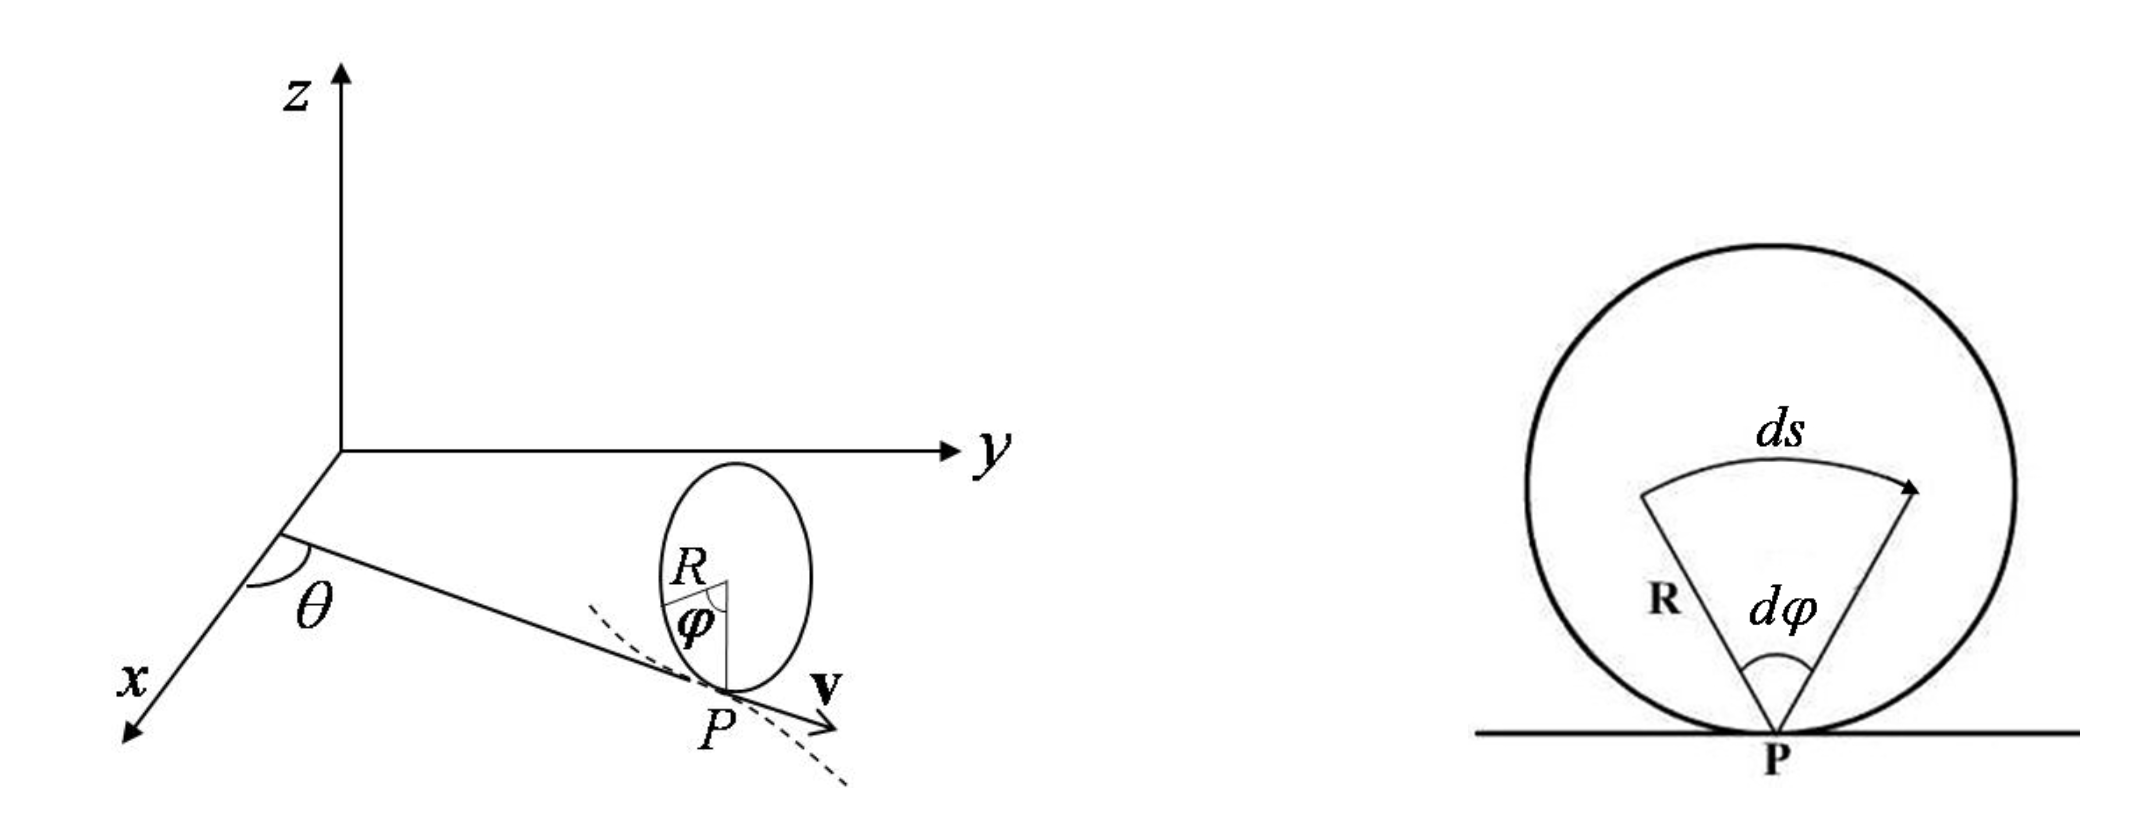
\includegraphics[width=2.8in]{Figuras/RuedaSinDeslizar.png} 
   		         \end{figure}
}
  
\end{document}

%%%%% Diapo 2
\section{Secci�n}
\frame{
  \frametitle{T�tulo transparencia}
  \begin{itemize}  
  	\item<1-> 
   \end{itemize}
}
%%%%% Diapo 2
\section{Secci�n}
\frame{
  \frametitle{T�tulo transparencia}
  \begin{itemize}  
  	\item<1-> 
   \end{itemize}
}
%%%%% Diapo 2
\section{Secci�n}
\frame{
  \frametitle{T�tulo transparencia}
  \begin{itemize}  
  	\item<1-> 
   \end{itemize}
}
%%%%% Diapo 2
\section{Secci�n}
\frame{
  \frametitle{T�tulo transparencia}
  \begin{itemize}  
  	\item<1-> 
   \end{itemize}
}

%%%%% Diapo Fin
\section{Recapitulando}
\frame{
  \frametitle{Recapitulando}
En presentaci�n consideramos
  \begin{enumerate}
  \item<1->
    \end{enumerate}
}
